
\chapter*{Licencia y Copyright}
\addcontentsline{toc}{chapter}{Licencia y Copyright}

{\noindent
Copyright \copyright\ Rosita Wachenchauzer <rositaw@gmail.com> \\
Copyright \copyright\ Margarita Manterola <margamanterola@gmail.com> \\
Copyright \copyright\ Maximiliano Curia <maxy@gnuservers.com.ar> \\
Copyright \copyright\ Marcos Medrano <mmedrano@fi.uba.ar> \\
Copyright \copyright\ Nicolás Paez <nicopaez@computer.org> \\
Copyright \copyright\ Diego Essaya <dessaya@gmail.com> \\
Copyright \copyright\ Dato Simó <dato@net.com.org.es> \\
}

\begin{center}
\noindent
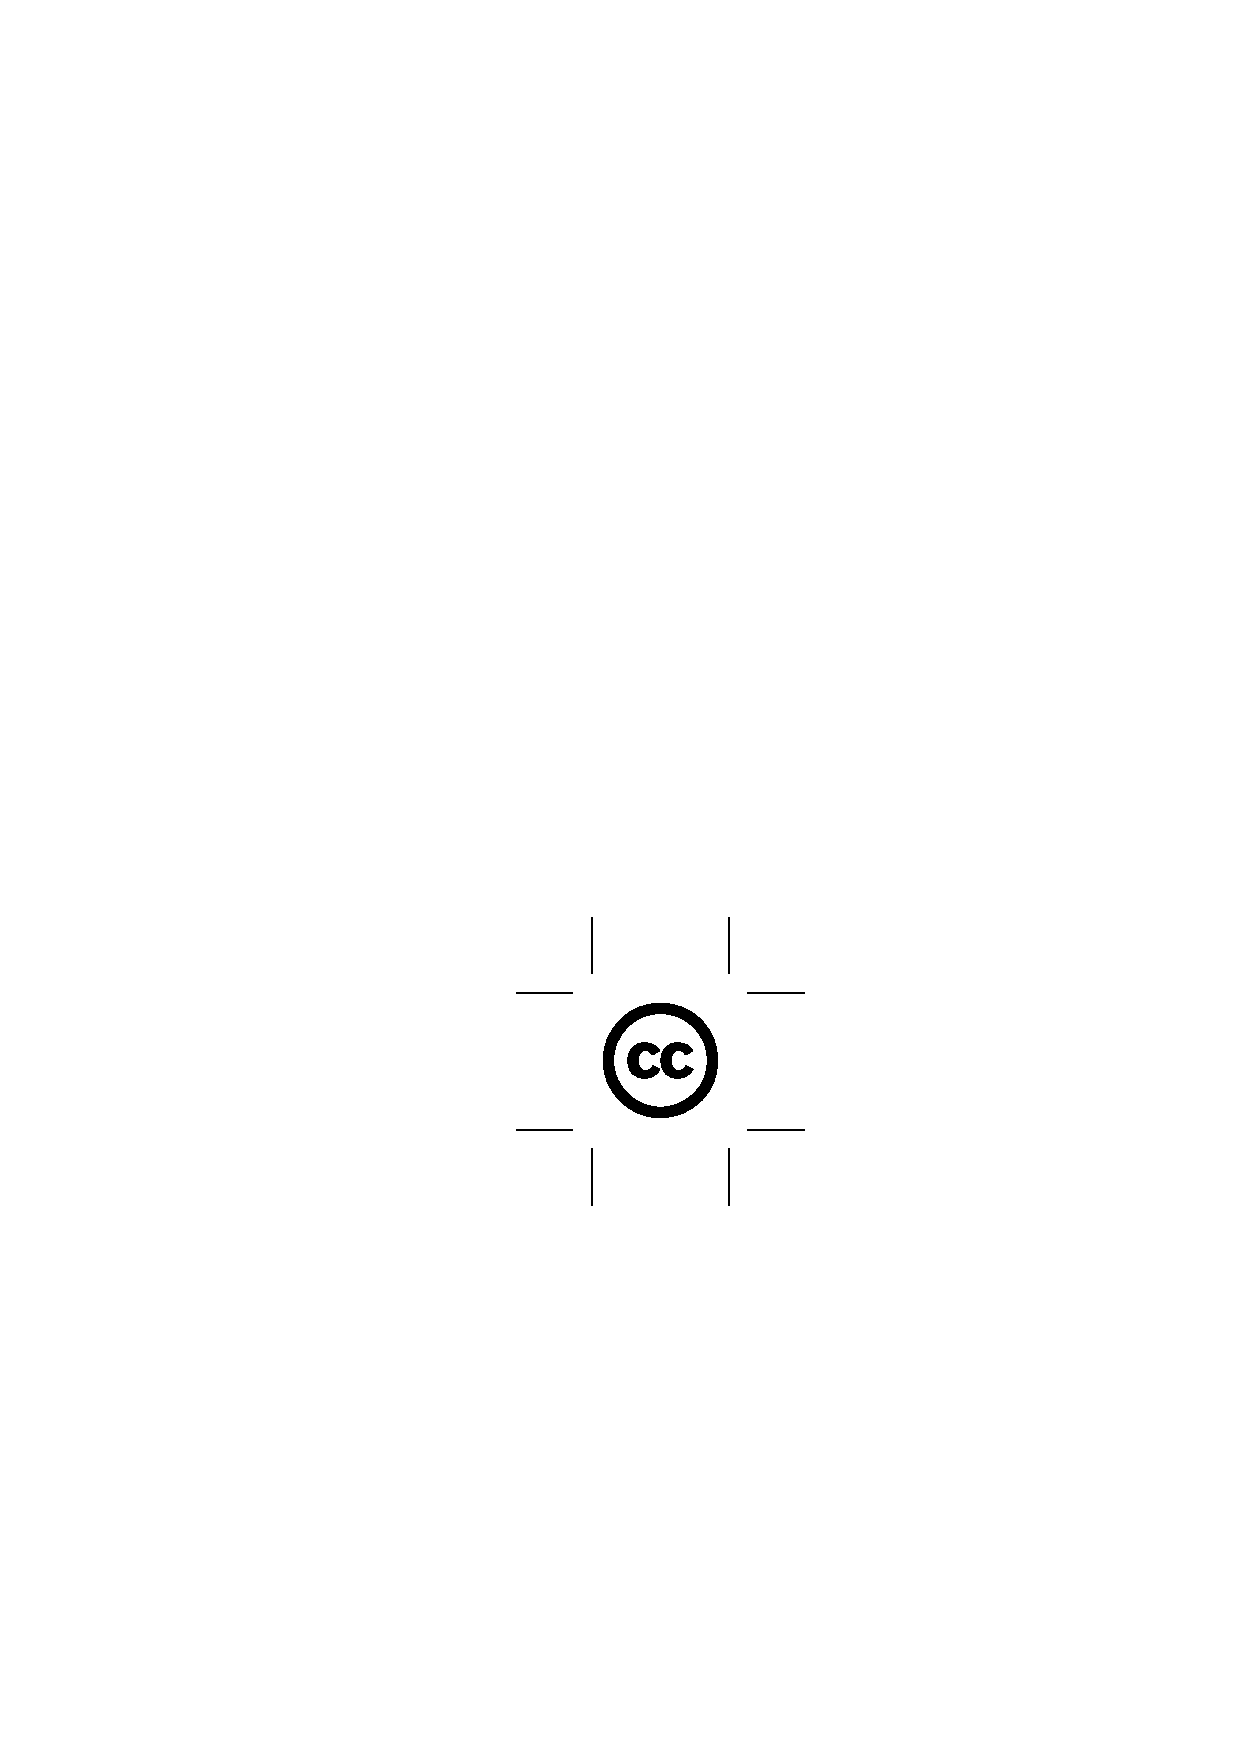
\includegraphics[height=1.5cm]{graficos/cc/cc}
\hspace{0.5cm}
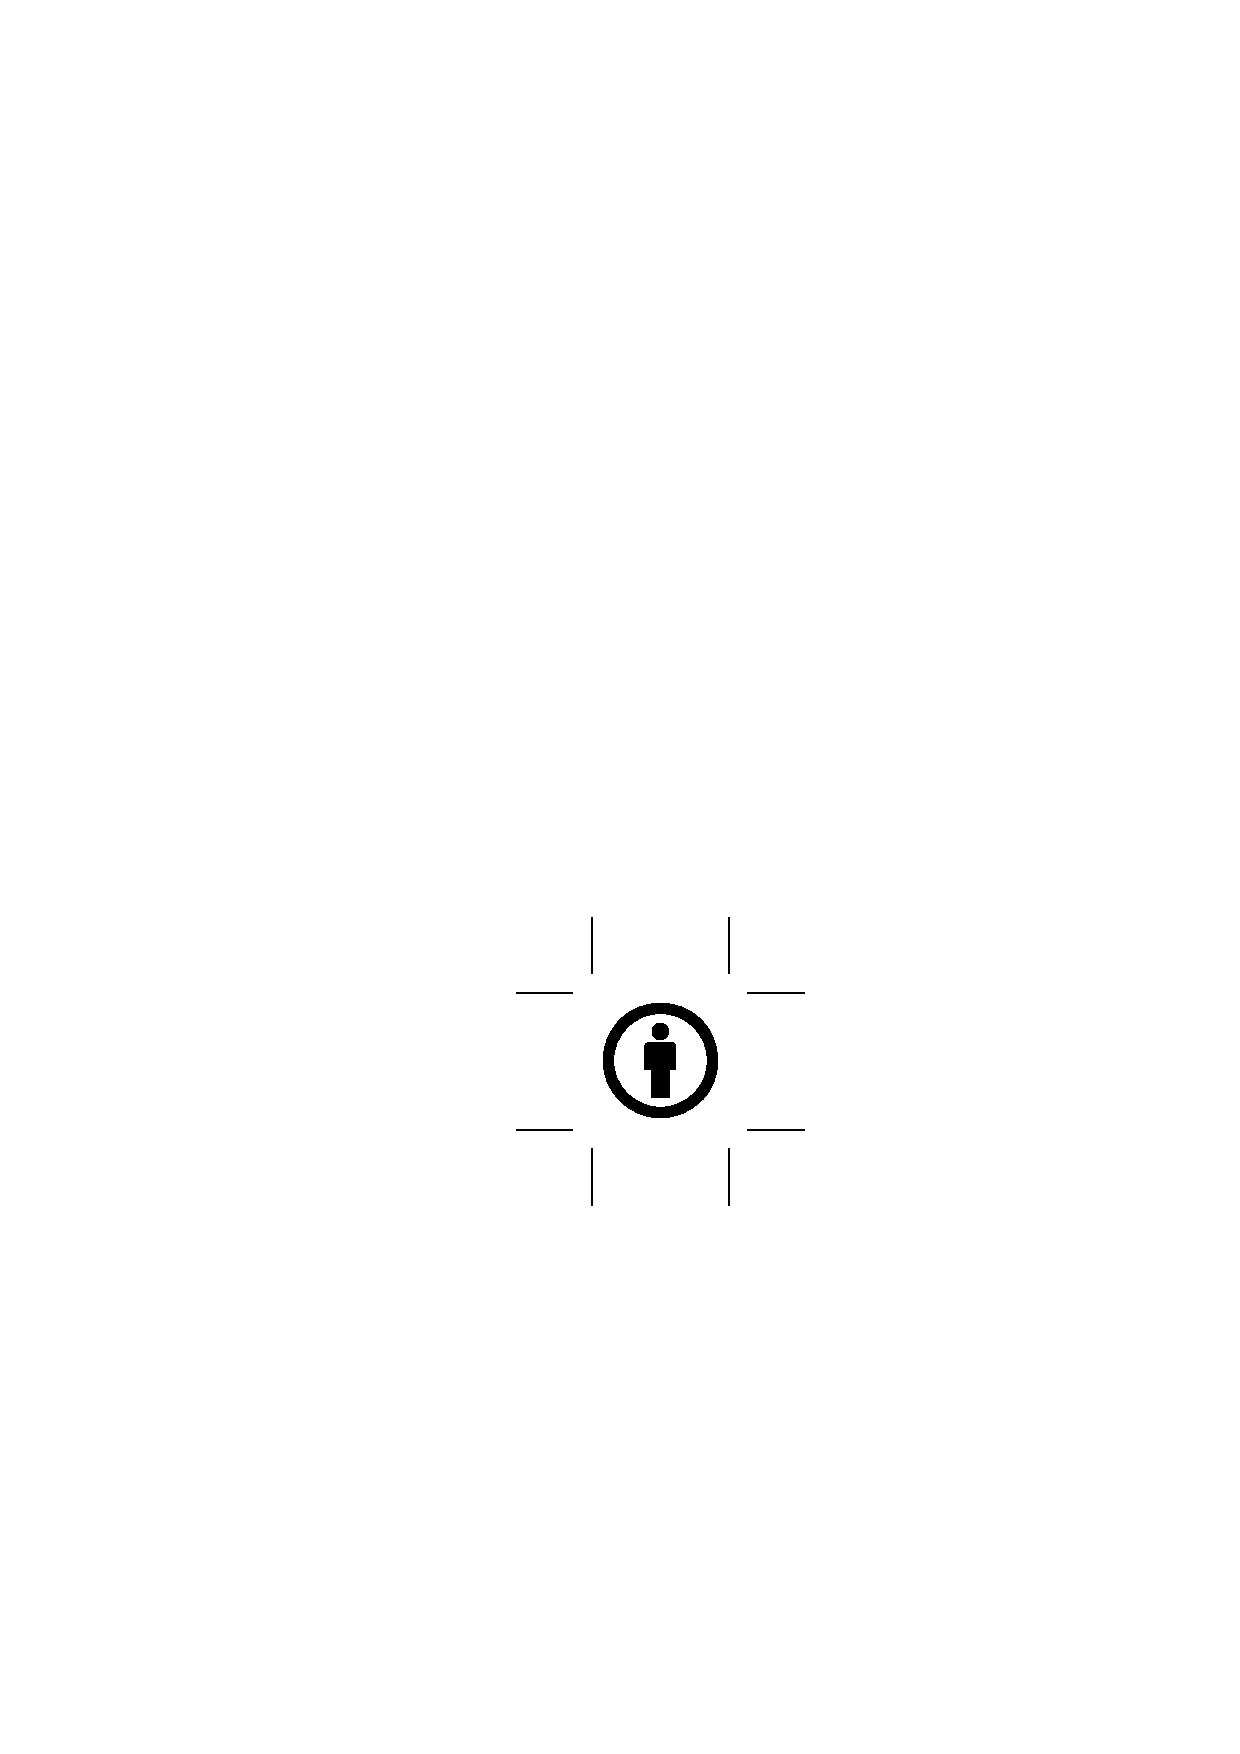
\includegraphics[height=1.5cm]{graficos/cc/by}
\hspace{0.5cm}
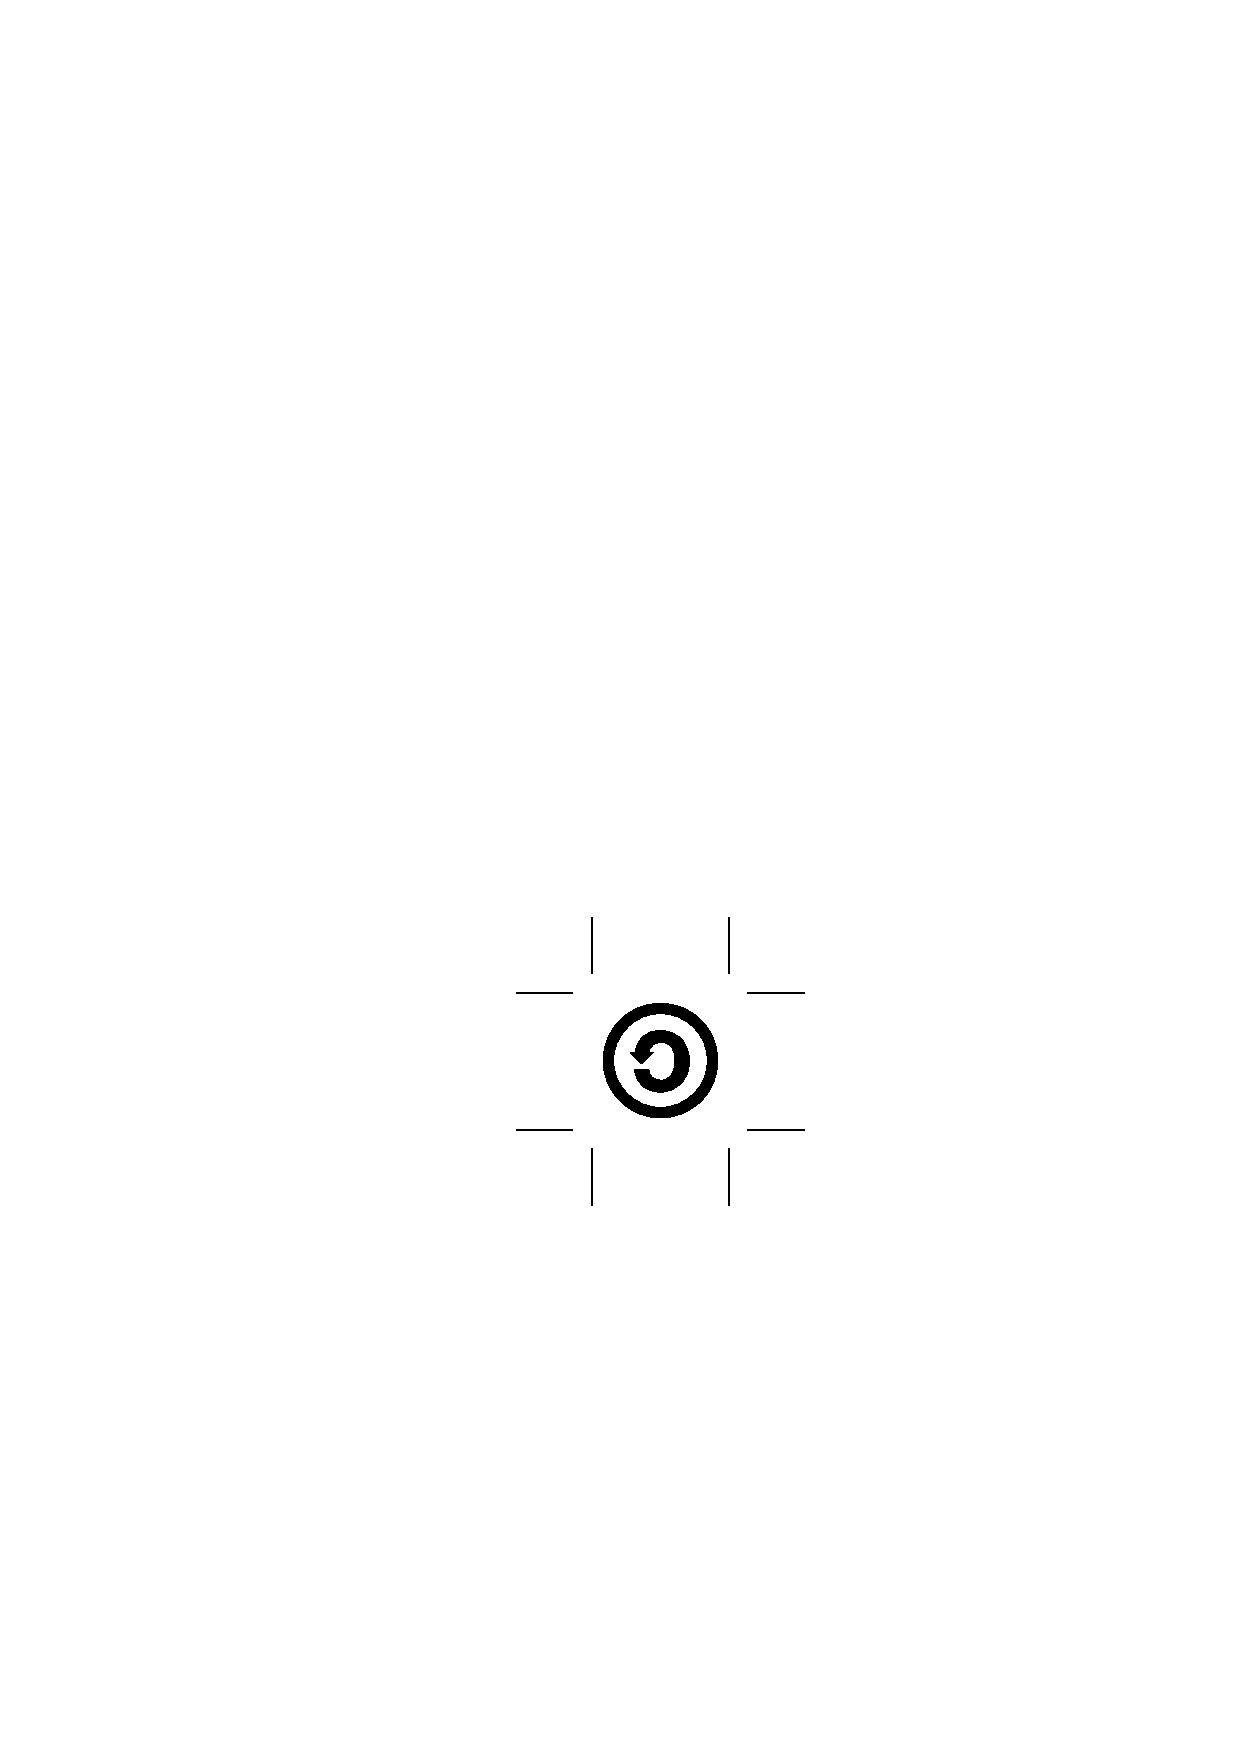
\includegraphics[height=1.5cm]{graficos/cc/sa}
\end{center}

Esta obra se distribuye bajo la
\href{http://creativecommons.org/licenses/by-sa/4.0/deed.es}{Licencia Creative
Commons Atribución-CompartirIgual 4.0 Internacional}.

Los íconos utilizados fueron diseñados por
\href{http://www.freepik.com/}{Freepik}.

El logo de Python es una marca registrada de la
\href{https://www.python.org/psf/}{Python Software Foundation}.

La publicidad de Cacao Droste es de dominio público, y fue descargada de
\href{http://en.wikipedia.org/wiki/Image:Droste.jpg}{Wikipedia}.
